\documentclass[conference]{IEEEtran}
\IEEEoverridecommandlockouts
% The preceding line is only needed to identify funding in the first footnote. If that is unneeded, please comment it out.
\usepackage{cite}
\usepackage{amsmath,amssymb,amsfonts}
\usepackage{algorithmic}
\usepackage{graphicx}
\graphicspath{{./figures/}}
\usepackage{textcomp}
\usepackage{booktabs}
\usepackage[table,xcdraw]{xcolor}
\usepackage[utf8]{inputenc}
\usepackage[T1]{fontenc}
\usepackage[english]{babel}
\usepackage{microtype} % optional, for aesthetics
\usepackage{tabularx} % nice to have
\usepackage{booktabs} % necessary for style
\usepackage{graphicx}
\graphicspath{{./figures/}}
\usepackage{listings}
\usepackage{multirow}
\usepackage{hhline}
\usepackage{caption}
\usepackage{makecell}
\usepackage{ragged2e}
\usepackage{parskip}
\usepackage{wrapfig}
\usepackage{array}
\usepackage{float}
\usepackage{lipsum}
\usepackage{subcaption}
\usepackage[linesnumbered,ruled]{algorithm2e}
\usepackage{courier}
%\usepackage{hyperref}
%\hypersetup{colorlinks=false,allcolors=false,bookmarks=false}
\usepackage{nohyperref}
\usepackage{url}
\usepackage{listings}
\usepackage{float}
\lstset{
    basicstyle=\ttfamily,
    frame=none, 
    breaklines=true,
    numbers=left,
    xleftmargin=1.5em,
    framexleftmargin=0em,
    emphstyle=\textbf,
    float=t
}
\lstdefinestyle{ocl}{
    emph={
        context, inv
    }
}
\lstdefinestyle{cbp}{
    basicstyle=\ttfamily\scriptsize,
    emph={
        session, create, type,
        set, to, add, hire
    }
}
\lstdefinestyle{xmi}{
    basicstyle=\ttfamily\scriptsize,
    emph={
        Node, children
    }
}
\lstdefinestyle{xml}{
    basicstyle=\ttfamily\scriptsize,
    emph={
        register, create, add, to, resource, at,
        from, eattribute, remove, ereference,
        set, unset, session, Roy, Jen,
        Moss, Richmond
    }
}
\lstdefinestyle{java}{
    basicstyle=\ttfamily\scriptsize,
    emph={
        case, $unset$,
        instanceof, else, if, void,
        new, UnsetEAttributeEvent,
        UnsetEReferenceEvent,
        @override, public, class, extends
    }
}
\lstdefinestyle{eol}{
    basicstyle=\ttfamily\scriptsize,
    emph={
        var, new, for, in, create, set, with, type, at,
        unset, to, add, remove, delete, register, move,
        from, position, from, move-within, session, comp, composite, \.
    }
}


\def\BibTeX{{\rm B\kern-.05em{\sc i\kern-.025em b}\kern-.08em
    T\kern-.1667em\lower.7ex\hbox{E}\kern-.125emX}}


\begin{document}

\title{Towards Visualising Change-based Models
%    *\\
%{\footnotesize \textsuperscript{*}Note: Sub-titles are not captured in Xplore and should not be used}
%\thanks{Identify applicable funding agency here. If none, delete this.}
}

\author{
    \IEEEauthorblockN{Alfa Yohannis\IEEEauthorrefmark{1}\IEEEauthorrefmark{3}, Horacio Hoyos Rodriguez\IEEEauthorrefmark{1}, Fiona Polack\IEEEauthorrefmark{2}, Dimitris Kolovos\IEEEauthorrefmark{1}}
    \IEEEauthorblockA{\IEEEauthorrefmark{1}Department of Computer Science, University of York
        \\alfa.yohannis@merahputih.id, horacio\_hoyos\_rodriguez@ieee.org, dimitris.kolovos@york.ac.uk}
    \IEEEauthorblockA{\IEEEauthorrefmark{2}School of Computing and Maths, Keele University, United Kingdom
        \\f.a.c.polack@keele.ac.uk}
    \IEEEauthorblockA{\IEEEauthorrefmark{3}Department of Computer Science, Kalbis Institute, Indonesia}
}
\maketitle

\begin{abstract}
This paper extends our previous work on change-based model persistence and 
demonstrates a tool that can replay the construction change-based model. The tool 
takes a change-based persistence file as input and plays it 
in the form of evolving diagrams reflecting the changes applied to 
the model.


\end{abstract}

\begin{IEEEkeywords}
visualization, change-based persistence, model evolution, BPMN2, model-driven engineering,
replay, animation
\end{IEEEkeywords}

\section{Introduction}
\label{sec:introduction}
In \cite{DBLP:conf/models/YohannisKP17}, we explored the concept of change-based persistence for models conforming
to object-oriented metamodelling architectures, such as MOF and Ecore. 
We also demonstrated a prototype (EpsilonLabs CBP\footnote{\url{https://github.com/epsilonlabs/emf-cbp}}), which enables persisting EMF models 
as sequences of changes (as opposed to snapshots of their state in XMI), which was 
further evaluated and extended in 
\cite{yohannis2018towards,DBLP:conf/models/YohannisRPK18,yohannis2018efficient}.

In this paper, we extend our previous work on change-based persistence (CBP) of models conforming to the MOF/EMF metamodelling architectures
\cite{DBLP:conf/models/YohannisKP17,yohannis2018towards,DBLP:conf/models/YohannisRPK18,yohannis2018efficient}
by contributing a tool that can visualise changes that have been applied to construct a model. 
Our tool takes a change-based model as input and constructs an animation of the changes it comprises. 

The rest of the paper is structured as follows. 
Section \ref{sec:change-based_persistence} provides an overview of our previous work on change-based model persistence. 
Section \ref{sec:visualising_model_construction} discusses our approach to using change-based persistence to visualise model construction. 
Section \ref{sec:evaluation} presents the evaluation of our approach. 
Section \ref{sec:related_work} provides an overview of related work, and
Section \ref{sec:conclusions_and_future_work} concludes with a discussion on directions for future work.

\section{Change-based Persistence}
\label{sec:change-based_persistence}

Instead of persisting snapshots of models as commonly practised in model-driven engineering, 
change-based model persistence persists the complete editing history of changes. 
This means that all changes applied to a model are recorded so that they can be re-used for other purposes. 

\begin{figure}[h]
    \centering
    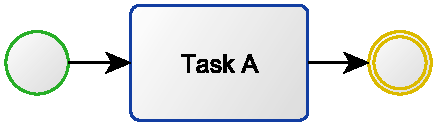
\includegraphics[width=0.5\linewidth]{bpmn2}
    \caption{A simple BPMN2 model.}
    \label{fig:bpmn2}
\end{figure}

Let's say that Bob developed a simple BPMN2 model in Figure \ref{fig:bpmn2}. If the model is persisted in a state-based format, 
the persistence produces an XMI file (simplified) as in Listing \ref{lst:bpmn2_xmi}.
This type of persistence only preserves the eventual state of the model,  
losing the detailed information of changes executed by Bob to construct the model. In contrast, 
if we record all the changes made by Bob and persist them into a CBP file, we can obtain a list of change events in Listing \ref{lst:bpmn2_cbp}.
In this list, the CBP file is pseudo-formatted to improve readability, but in implementation, the file is persisted in an XML-like format.
Replaying these recorded changes produces a model with the same eventual state as in Figure \ref{fig:bpmn2} and Listing \ref{lst:bpmn2_xmi}.

\vspace{-15pt}
\begin{lstlisting}[style=eol,numbersep=1pt,caption={A BPMN2 model in Figure \ref{fig:bpmn2} persisted in simplified XMI.},label=lst:bpmn2_xmi]
<process id="e1" name="Process 1">
 <startEvent id="e2">
   <outgoing>e6</outgoing>
 </startEvent>
 <endEvent id="e4">
   <incoming>e7</incoming>
 </endEvent>
 <task id="e5" name="Task A">
   <incoming>e6</incoming>
   <outgoing>e7</outgoing>
 </task>
 <sequenceFlow id="e6" sourceRef="e2" targetRef="e5"/>
 <sequenceFlow id="e7" sourceRef="e5" targetRef="e4"/>
</process>
\end{lstlisting}

From Listing \ref{lst:bpmn2_cbp}, we can know the sequence of changes made by Bob to construct the model. We can also identify that Bob made invalid changes 
that connect SequenceFlow \texttt{e3} from EndEvent \texttt{e4} to StartEvent \texttt{e2} 
(no SequenceFlow is allowed to come out from an EndEvent or enter a StartEvent) (lines 10-11) 
which he deleted in the following changes (lines 13-17). 
Such phenomenon might not be identified if we persist the model in state-based format. 

\vspace{-15pt}
\begin{lstlisting}[style=eol,numbersep=5pt,caption={The pseudo-formatted CBP of the model in Figure \ref{fig:bpmn2}.},label=lst:bpmn2_cbp]
create e1 type Process
set e1.name to "Process 1"
create e2 type StartEvent
add e2 to e1.flowElements at 0
create e3 type SequenceFlow
set e3.name from to "Sequence Flow 1"
add e3 to e1.flowElements at 1
create e4 type EndEvent
add e4 to e1.flowElements at 0
add e3 to e2.incoming at 0
add e3 to e4.outgoing at 0
add e1 to resource at 0
remove e3 from e2.outgoing at 0 composite c1
remove e3 from e4.incoming at 0 composite c1
unset e3.name from "Sequence Flow 1" to null composite c1
remove e3 from e1.flowElements at 1 composite c1
delete e3 type SequenceFlow composite c1
create e5 type Task
set e5.name from to "Task 1"
add e5 to e1.flowElements at 2
create e6 type SequenceFlow
add e6 to e2.outgoing at 0
add e6 to e5.incoming at 0
add e6 to e1.flowElements at 3
create e7 type SequenceFlow
add e7 to e5.outgoing at 0
add e7 to e4.incoming at 0
add e7 to e1.flowElements at 4
set e5.name to "Task A"
\end{lstlisting}

While persisting all these changes is perceived too excessive as it requires more storage space \cite{DBLP:conf/models/YohannisRPK18}, 
in some conditions, it is desirable especially when we want to perform model analytics, 
such as understanding model evolution, identifying model editing/language usage patterns, etc. \cite{DBLP:conf/models/YohannisKP17}. 
Moreover, CBP can also drastically speed up model comparison \cite{yohannis2018efficient}.

Trying to understand changes executed by Bob in Listing \ref{lst:bpmn2_cbp} may require extra cognitive effort 
as one who tries to comprehend it needs to build a mental model and emulate the changes in their mind.
One solution to reduce the required cognitive effort is by providing a visualisation tool.
With the tool, they can replay the model construction and observe what kind of changes have been made by Bob.

\section{Visualising Model Construction}
\label{sec:visualising_model_construction}
For the reasons we have exposed, we have built CBP-Player, a prototype\footnote{Project and demo can be found at \url{https://github.com/epsilonlabs/emf-cbp/tree/master/CBPPlayer} 
    and \url{https://alfa-ryano.github.io/visualization.html}},
that visualises the construction of change-based models.
It is a JavaScript application and uses the mxGraph diagramming library
 \cite{mxgraph2019mxgraph} for displaying graphical representations of the evolving model. 

\subsection{Process}
\label{sec:process}
Figure \ref{fig:process} shows the process of drawing a model in CBP-Player. 
The process consists of three phases: Loading, Building, and Drawing.  
In the Loading phase, the CBP-Player loads a CBP file as a sequence of change events in memory. 
It also loads the metamodel of the change-based model. 
The metamodel\footnote{For now, the metamodel is still defined from scratch in Javascript. Further extension is required to load metamodel from Ecore files.} 
defines the model that will be constructed by the Building phase.

\begin{figure}[h]
    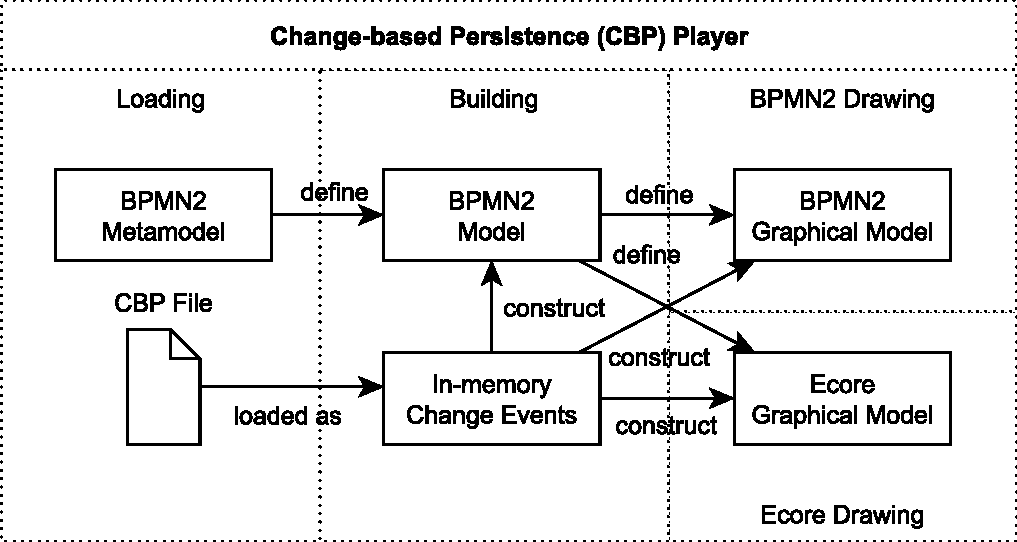
\includegraphics[width=\linewidth]{process}
    \caption{The process to visualise model construction using change-based persistence.}
    \label{fig:process}
\end{figure}

In the Building and Drawing phases, the CBP-Player plays the loaded change events one-by-one emulating the construction of the model in the CBP file.
This construction also computes the values required to draw the model's graphical representation.
For example, the shifting of elements' indexes caused by the deletion of an element in a containing feature
in order to label edges, or determining the types of edges to represent features. 

When executing a change event, besides applying the change to construct an abstract/semantic model, 
the change is also reflected to a graphical model. Currently, 
the prototype is designed to have more than one model drawer to reflect changes to different graphical models. 
In Figure \ref{fig:process}, we have two drawings 
which allow viewing a model construction in two perspectives: here, BPMN2 and 
object-diagram-like notation that visualises Ecore models in a graph/tree structure 
(further we refer this as Ecore).

\subsection{Implementation}
\label{sec:implementation}
Figure \ref{fig:class_diagram} depicts the simplified class diagram 
of the implementation of the CBP-Player. The main class, \texttt{CBP-Player}, has methods \texttt{load},
\texttt{play}, and \texttt{stop} to load and control the play of a CBP file.

\begin{figure}[h]
    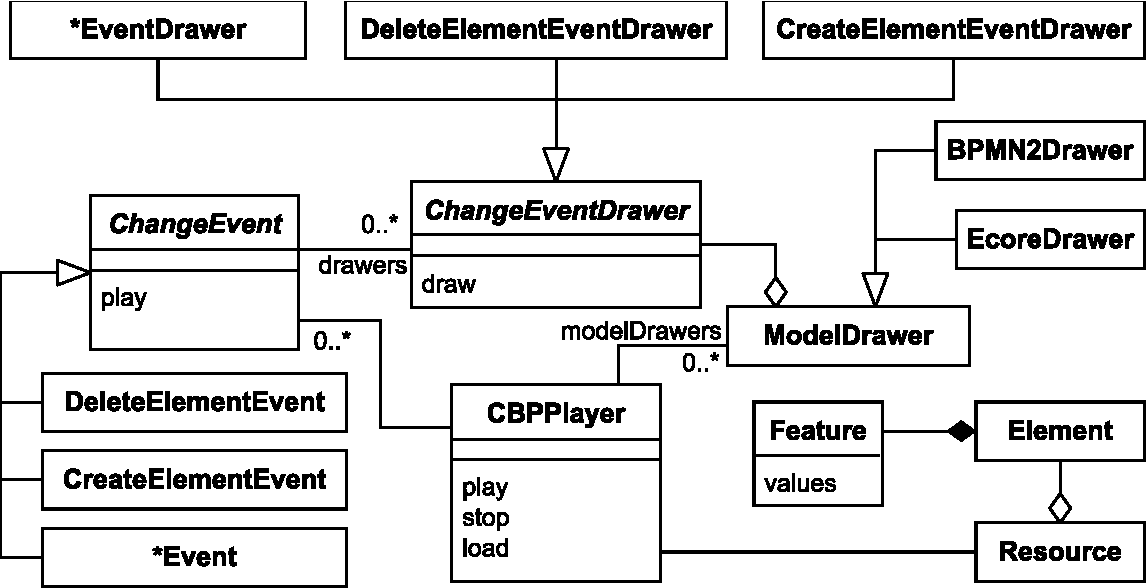
\includegraphics[width=\linewidth]{class_diagram}
    \caption{The simplified class diagram of the CBP-Player implementation.}
    \label{fig:class_diagram}
\end{figure}

\begin{figure}
  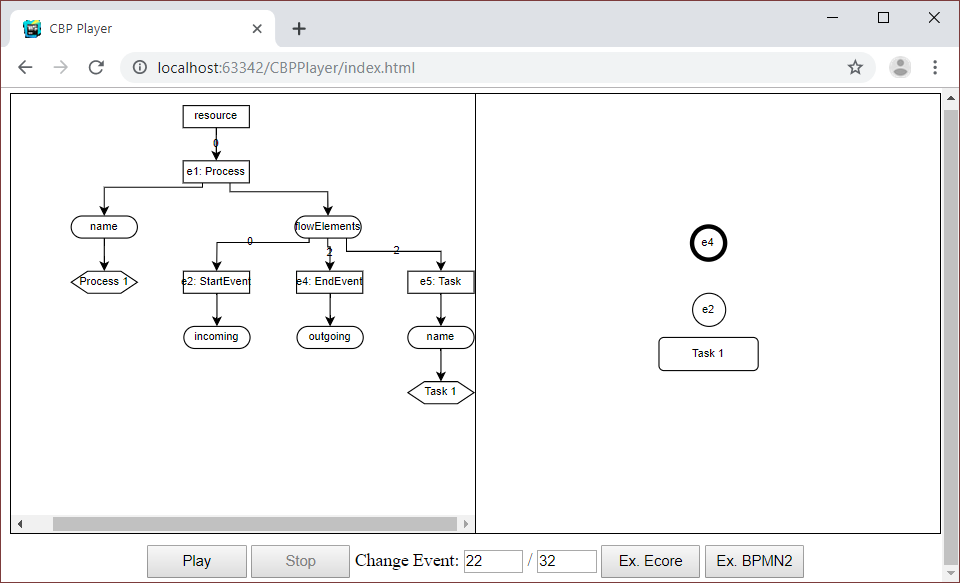
\includegraphics[width=\linewidth]{prototype}
  \caption{The application of CBP-Player.}
  \label{fig:implementation}
\end{figure}

\begin{figure*}
  \begin{subfigure}[t]{0.2\linewidth}
    \centering
    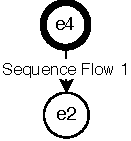
\includegraphics[width=\linewidth]{bpmn2_12}
    \caption{BPMN2 model at line 12 in Listing \ref{lst:bpmn2_cbp}}
    \label{fig:bpmn2_12}
  \end{subfigure}
  \hfill
  \begin{subfigure}[t]{0.2\linewidth}
    \centering
    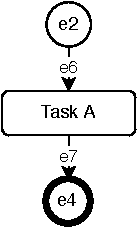
\includegraphics[width=\linewidth]{bpmn2_32}
    \caption{BPMN2 model at line 29 in Listing \ref{lst:bpmn2_cbp}}
    \label{fig:bpmn2_29}
  \end{subfigure}
  \hfill
  \begin{subfigure}[t]{0.40\linewidth}
    \centering
    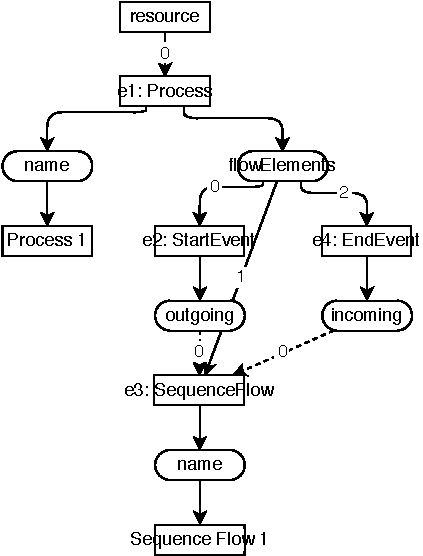
\includegraphics[width=\linewidth]{ecore_12}
    \caption{Ecore model at line 12 in Listing \ref{lst:bpmn2_cbp}}
    \label{fig:ecore_12}
  \end{subfigure}
  \\
  \begin{subfigure}[t]{\linewidth}
    \centering
    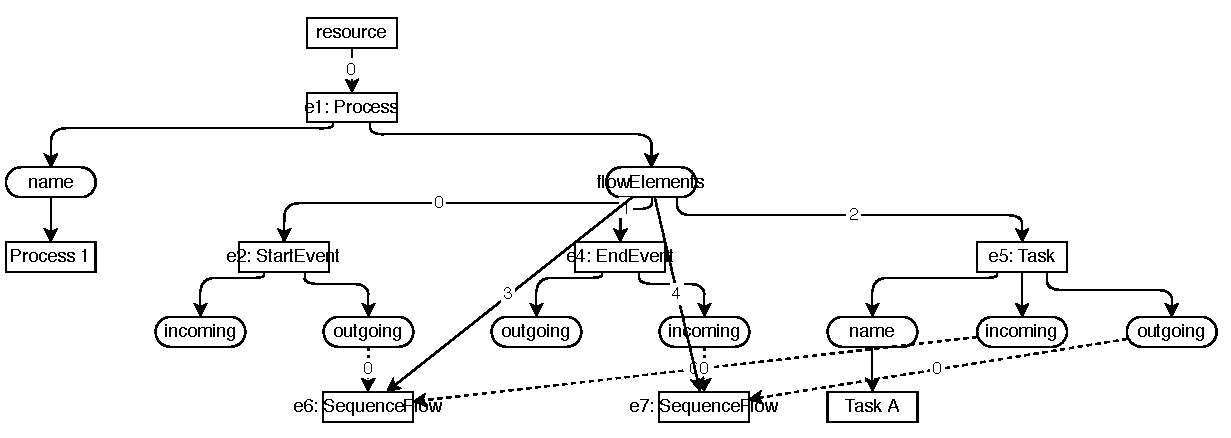
\includegraphics[width=\linewidth]{ecore_32}
    \caption{Ecore model at line 29 in Listing \ref{lst:bpmn2_cbp}}
    \label{fig:ecore_29}
  \end{subfigure}
  \caption{The graphical models produced by the prototype during the construction of the model in Figure \ref{fig:bpmn2}.}
  \label{fig:prototype}
\end{figure*}

When initialising, the \texttt{CBPPlayer} registers all kinds of \texttt{ModelDrawer} that are going to be used. 
In Figure \ref{fig:class_diagram}, we use \texttt{EcoreDrawer} and \texttt{BPMN2Drawer} classes as examples for the model drawers. 
Both classes are derived from \texttt{ModelDrawer} class. This \texttt{ModelDrawer} class consists of 
different extension classes of the \texttt{ChangeEventDrawer} class. Each extension class determines
what kind of drawing operations should be executed on the graphical model if an instance of \texttt{ChangeEvent} is executed.
For example, when the play method of the \texttt{DeleteElementEventDrawer} class is executed,
it removes an element from the graphical model. The instance of this class should be registered to
its corresponding \texttt{ChangeEvent}, in this case, class \texttt{DeleteElementEvent}. 
If the instance of this \texttt{ChangeEvent} plays, it also executes the \texttt{draw} method of 
the \texttt{ChangeEventDrawer} instances registered to it. Thus, if an element is deleted from an abstract model,
the corresponding element is also deleted in its graphical representation. 

While executing the load method, a CBP file is loaded into memory,  
a list of \texttt{ChangeEvent} (changeEvents), and a corresponding \texttt{ChangeEventDrawer} is 
registered to each change event. 
When \texttt{CBP-Player} plays this \texttt{changeEvents}, it iterates throughout the list and executes  
the \texttt{play} method of each change event emulating the construction of a model. 
After executing each \texttt{play} method, the \texttt{draw} method of 
the corresponding registered \texttt{ChangeEventDrawer} is also executed to draw the model's graphic.
Classes \texttt{Resource}, \texttt{Element}, and \texttt{Feature} are used as internal data structures 
for constructing the abstract model.

\subsection{Application}
\label{sec:application}
To obtain the change-based model in Listing \ref{lst:bpmn2_cbp}, firstly, we had to modify
the Eclipse BPMN2 Modeler \cite{eclipse2019bpmn2}. In particular, we added \texttt{ChangeEventAdapter} \cite{epsilonlabs2019changeeventadapter}
of the EpsilonLabs CBP \cite{DBLP:conf/models/YohannisKP17}  to the \texttt{Bpmn2Resource}'s \texttt{eAdapters}
in the Eclipse BPMN2 Modeler. The said adapter can capture every change made to a model through the modeller.
We then created the model in Figure \ref{fig:bpmn2} by following the course of changes in Listing \ref{lst:bpmn2_cbp}, and saved the model, producing XMI and CBP files such as those 
in Listings \ref{lst:bpmn2_xmi} and \ref{lst:bpmn2_cbp}. 


We have built a simple application in which we employ the CBP-Player (Figure \ref{fig:implementation}). The application can visualise the construction of a BPMN2 model using two notations: an object-diagram-like notation, and the standard BPMN2 graphical syntax. 
To demonstrate the application, we feed it with the produced CBP file.
The application loads the change events in the CBP file into memory and replays them one-by-one. Every time a change event is replayed, it is also reflected in the two diagrams. 

In the object diagram perspective, as displayed in Figure \ref{fig:ecore_12}, 
elements and values are represented with rectangles, features are depicted in rounded rectangles, and containment/non-containment relationships are represented with solid/dashed directed edges. Solid directed edges also represent ownership between elements and their features. Numbers on the edges indicate the indexes of the elements in their containers. 

Figure \ref{fig:prototype} shows the graphical models displayed by the prototype. Figures \ref{fig:ecore_12} and \ref{fig:bpmn2_12} show the object diagram and BPMN2 diagram at the time when edge \texttt{e3} is about to be removed (Listing \ref{lst:bpmn2_cbp}, line 12). In Figure \ref{fig:ecore_12}, we can notice there is element \texttt{e1} with type \texttt{Process} contained by the resource at index 0. The element has a single-valued feature \texttt{name} with value ``Process 1''. Element \texttt{e1} also has a multi-valued feature \texttt{flowElements} that contains three other elements, \texttt{e2} with type \texttt{StartEvent}, \texttt{e3} with type \texttt{SequenceFlow}, and \texttt{e4} with type \texttt{EndEvent}, each at index 0, 1, and 3 respectively. Element \texttt{e3} has a feature \texttt{name} with value ``Sequence Flow 1''. This element is referenced by elements \texttt{e2}'s \texttt{incoming} and \texttt{e4}'s \texttt{outgoing} features.  

Figure \ref{fig:bpmn2_12} displays the model in BPMN2; the state of the model in the object diagram perspective is hidden from users. In the figure, we can notice a \texttt{SequenceFlow} with name ``Sequence Flow 1'' wrongly connects \texttt{EndEvent} \texttt{e2} to \texttt{StartEvent} \texttt{e1}. No \texttt{SequenceFlow} is allowed to leave an \texttt{EndEvent} or enter a \texttt{StartEvent}. Later, the \texttt{SequenceFlow} is removed from the model (Listing \ref{lst:bpmn2_cbp} lines 13-17).          

Figures \ref{fig:bpmn2_29} and \ref{fig:ecore_29} show the diagrams after all changes have been applied. In Figure \ref{fig:bpmn2_29}, the diagram does not contain the \texttt{SequenceFlow} with name ``Sequence Flow 1'' anymore. It is replaced with a Task ``Task A'' and two \texttt{SequenceFlow} \texttt{e6} and \texttt{e7} in the correct direction. Figure \ref{fig:ecore_29} shows the same model but displayed in the object diagram perspective. 

\section{Related Work}
\label{sec:related_work}
Some tools are available to visualise Ecore-based models. 
EcoreTools \cite{eclipse2019ecoretools} is a tool to define metamodels graphically while other tools such as
Eugenia \cite{Kolovos2017} and Sirius \cite{eclipse2019sirius} are used 
to define the visual concrete syntax of models.
Nevertheless, these tools are not intended to visualise the evolution or changes of models. 
Visualisation of model evolution has been studied in different domain-specific
modelling languages for business processes \cite{fritscher2014visualizing}
and software \cite{Mattila:2016:SVT:2994310.2994327}. Work on visualising changes specific to Ecore-based models 
was performed by Maier et al. \cite{maier2015recording}. 
They used a state-based approach to persist different versions of a model.
Changes between versions were derived using EMF Compare \cite{eclipse2017compare}, 
a model differencing tool, and then presented 
in a timeline format with colour-coding used 
to identify changes between versions, e.g. a new element is coloured green
while other old elements are coloured grey. In contrast, our approach
exploits change-based persistence to obtain changes and visualise them in
the form of animation.

\section{Conclusions and Future Work}
\label{sec:conclusions_and_future_work}
This paper has presented an extension to the work of change-based model persistence
that aims at providing a tool, the CBP-Player, to visualise model construction. 
The tool takes a CBP file as input and plays it in the form of a graphical model,
emulating the changes applied to the persisted model. 
The tool is designed to be extensible to any types of visualisation that aim
to exploit the information contained in CBP. The tool itself is still at a prototype state. 
Some features that are planned to be added are visualising model differencing
and conflict detection and model metrics 
(number of elements, features, etc.) throughout the evolution of a model. We have not undertaken any performance evaluation in this work 
since performance is not the main goal of the current prototype.
To evaluate correctness, we have employed unit tests that exercise the features 
presented in this work. A systematic evaluation is required in later iterations 
to evaluate the performance, usefulness, and usability of the tool.


\section*{Acknowledgment}
This work was part supported by the European Commission via the CROSSMINER (project number 732223) and TYPHON (project number 780251) H2020 projects and through a scholarship managed by \emph{Lembaga Pengelola Dana Pendidikan Indonesia} (Indonesia Endowment Fund for Education).

%\section*{References}
\bibliographystyle{IEEETran}
\bibliography{references}

\end{document}
